\makeatletter
\def\input@path{{pwr-szablon/}}
\makeatother

\documentclass[aspectratio=169]{beamer}
\usepackage{polski}
\usetheme[lang=pl,hr=true]{NewPwr}
\graphicspath{{pwr-szablon/}{figures/}}

\usepackage{listings}
\usepackage{booktabs}
\usepackage{graphicx}

% DANE PROJEKTU
\author{Wojciech Bukała, Aleksander Łyskawa}
\title{Statystyczna analiza danych}
\subtitle{Analiza zbioru danych dotyczącego piłkarzy z najlepszych lig europejskich w sezonie 2025/26}
\institute{Politechnika Wrocławska}
\date{\today}

\begin{document}

\begin{frame}
    \maketitle
\end{frame}

\begin{frame}{Spis treści}
    \begin{enumerate}
        \item Zbiór danych
        \item Eksploracyjna analiza danych (EDA)
        \item Preprocessing
        \item Klasteryzacja zawodników (KMeans + PCA)
        \item Regresja — przewidywanie wartości rynkowej
        \item Klasyfikacja — przewidywanie pozycji zawodnika
        \item Weryfikacja hipotez statystycznych
    \end{enumerate}
\end{frame}

%%%
% Zbiór danych
%%%

\begin{frame}{Zbiór danych}
    Dataset zawiera profile piłkarzy oraz ich statystyki z przebiegu sezonu 2025-26, dla najlepszych lig europejskich. Zawiera:
    \begin{itemize}
        \item 4\,740 profili piłkarzy, plik \texttt{all\_player\_profiles.csv}
        \item 3\,749 rekordów ze statystykami, plik \texttt{all\_player\_stats.csv}
        \item Po złączeniu (inner join po \texttt{player\_id} i \texttt{league}): \textbf{3\,749 zawodników}
    \end{itemize}

    \vspace{0.3cm}

    Ligi europejskie brane pod uwagę:
    \begin{itemize}
        \item Premier League (Anglia), LaLiga (Hiszpania), Serie A (Włochy)
        \item Bundesliga (Niemcy), Ligue 1 (Francja), Eredivisie (Holandia)
        \item Liga Portugal (Portugalia), Super Lig (Turcja)
    \end{itemize}

    % \begin{block}{Uwaga}
    %     991 profili nie posiada statystyk meczowych — dotyczy głównie zawodników, którzy nie wystąpili w żadnym spotkaniu w danym sezonie (kontuzje, wypożyczenia, kadra rezerwowa).
    % \end{block}
\end{frame}

\begin{frame}[fragile]{Zbiór danych: \texttt{all\_player\_profiles.csv}}

    \begin{lstlisting}
profiles_df.info()  # 4 740 wierszy
    \end{lstlisting}

    \begin{tabular}{lccc}
        \toprule
        \textbf{\#} & \textbf{Column} & \textbf{Non-Null Count} & \textbf{Dtype} \\
        \midrule
        0 & player\_id & 4740 non-null & int64 \\
        1 & name & 4740 non-null & str \\
        2 & league & 4740 non-null & str \\
        3 & position & 4740 non-null & str \\
        4 & market\_value & 4068 non-null & float64 \\
        \bottomrule
    \end{tabular}

    \vspace{0.3cm}
    \begin{itemize}
        \item Pozycje: \textbf{F} (napastnik), \textbf{M} (pomocnik), \textbf{D} (obrońca), \textbf{G} (bramkarz)
        \item \texttt{market\_value}: \textbf{672 brakujące} wartości
    \end{itemize}
\end{frame}

\begin{frame}[fragile]{Zbiór danych: \texttt{all\_player\_stats.csv}}

    \begin{lstlisting}
stats_df.info()  # 3 749 wierszy, 17 kolumn
    \end{lstlisting}
    \small{
    \begin{tabular}{lcc|lcc}
        \toprule
        \textbf{Column} & \textbf{Non-Null} & \textbf{Dtype} & \textbf{Column} & \textbf{Non-Null} & \textbf{Dtype} \\
        \midrule
        player\_id & 3749 & int64 & rating & 3749 & float64 \\
        league & 3749 & str & total\_shots & 3749 & int64 \\
        appearances & 3749 & int64 & shots\_on\_target & 3749 & int64 \\
        matches\_started & 3749 & int64 & yellow\_cards & 3749 & int64 \\
        minutes\_played & 3749 & int64 & red\_cards & 3749 & int64 \\
        goals & 3749 & int64 & tackles & 3749 & int64 \\
        assists & 3749 & int64 & interceptions & 3749 & int64 \\
        expected\_goals & 3182 & float64 & saves & 3749 & int64 \\
        expected\_assists & 3723 & float64 & & & \\
        \bottomrule
    \end{tabular}}

    \vspace{0.4cm}
    
    \texttt{expected\_goals}: \textbf{567 braków (15\%)} i \texttt{expected\_assists}: \textbf{26 braków (0.7\%)}. Uzupełniane medianą w etapie preprocessingu.
    
\end{frame}

%%%
% EDA
%%%

\section{Eksploracyjna analiza danych}

\begin{frame}[c]
    \centering
    \vfill
    {\usebeamerfont{frametitle}\usebeamercolor[fg]{frametitle} Eksploracyjna analiza danych}
    \vfill
\end{frame}

\begin{frame}{Wykresy rozkładów}

    \begin{columns}[T]
        \begin{column}{0.3\textwidth}
            \begin{center}
                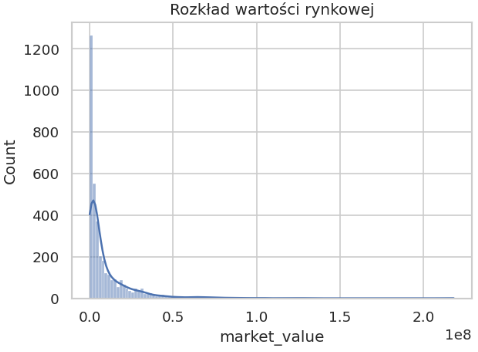
\includegraphics[width=0.95\textwidth]{figures/rozklad_wartosci_rynkowej.png}
                \textbf{Wartość rynkowa} - silnie prawostronny. Większość zawodników wyceniana poniżej 10M€, a tylko nieliczni przekraczają 100M€.               
            \end{center}
        \end{column}

        \begin{column}{0.3\textwidth}
            \begin{center}
                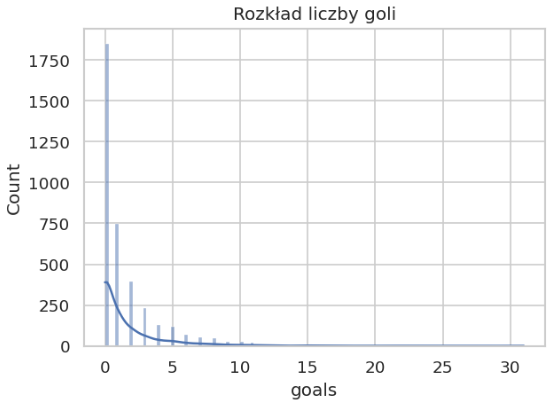
\includegraphics[width=0.95\textwidth]{figures/rozklad_liczby_goli.png}
                \textbf{Liczba goli} - bardzo skośna: ponad połowa zawodników (obrońcy, bramkarze) strzela 0 lub 1 gola.
            \end{center}
        \end{column}


        \begin{column}{0.3\textwidth}
            \begin{center}
                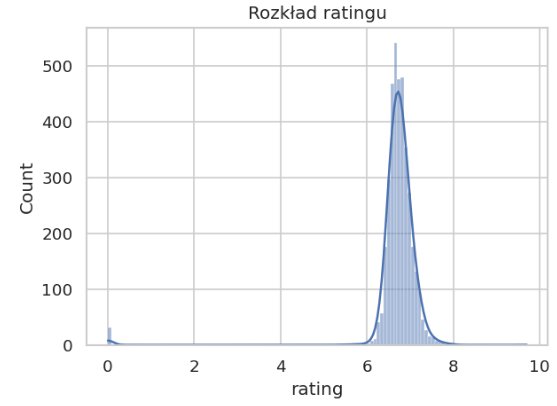
\includegraphics[width=0.95\textwidth]{figures/rozklad_ratingu.png}
                \textbf{Rating} - symetryczny, skoncentrowany wokół 6.7. Można sądzić, że skala ocen jest automatycznie centrowana.
            \end{center}
        \end{column}
    \end{columns}
\end{frame}

\begin{frame}{Wykresy rozkładów}

    \begin{columns}[T]
        \begin{column}{0.45\textwidth}
            \begin{center}
                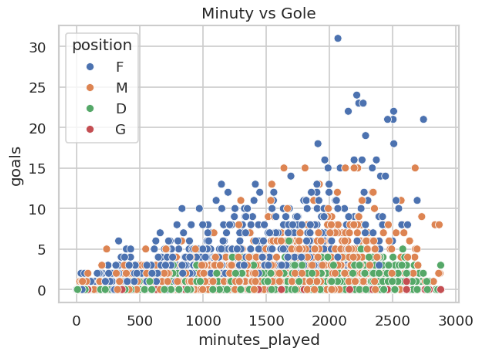
\includegraphics[width=1\textwidth]{figures/minuty_vs_gole.png}
            
                \textbf{Minuty vs Gole} - wyraźna zależność liniowa tylko dla napastników (F). Obrońcy i pomocnicy grają dużo, ale strzelają mało.
            \end{center}
        \end{column}

        \begin{column}{0.45\textwidth}
            \begin{center}
                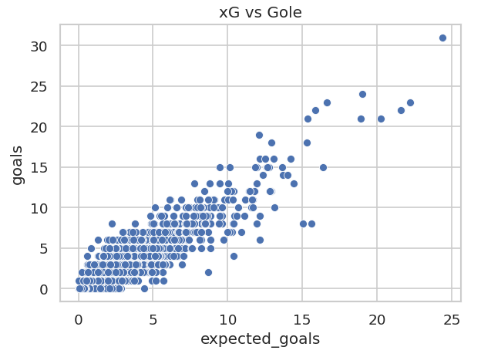
\includegraphics[width=1\textwidth]{figures/xg_vs_gole.png}
            
                \textbf{xG vs Gole} - wysoka korelacja ($r \approx 0.88$): model xG dobrze przewiduje rzeczywiste gole na poziomie populacji.
            \end{center}
        \end{column}

    \end{columns}
\end{frame}


\begin{frame}{Macierz korelacji}
    \begin{center}
        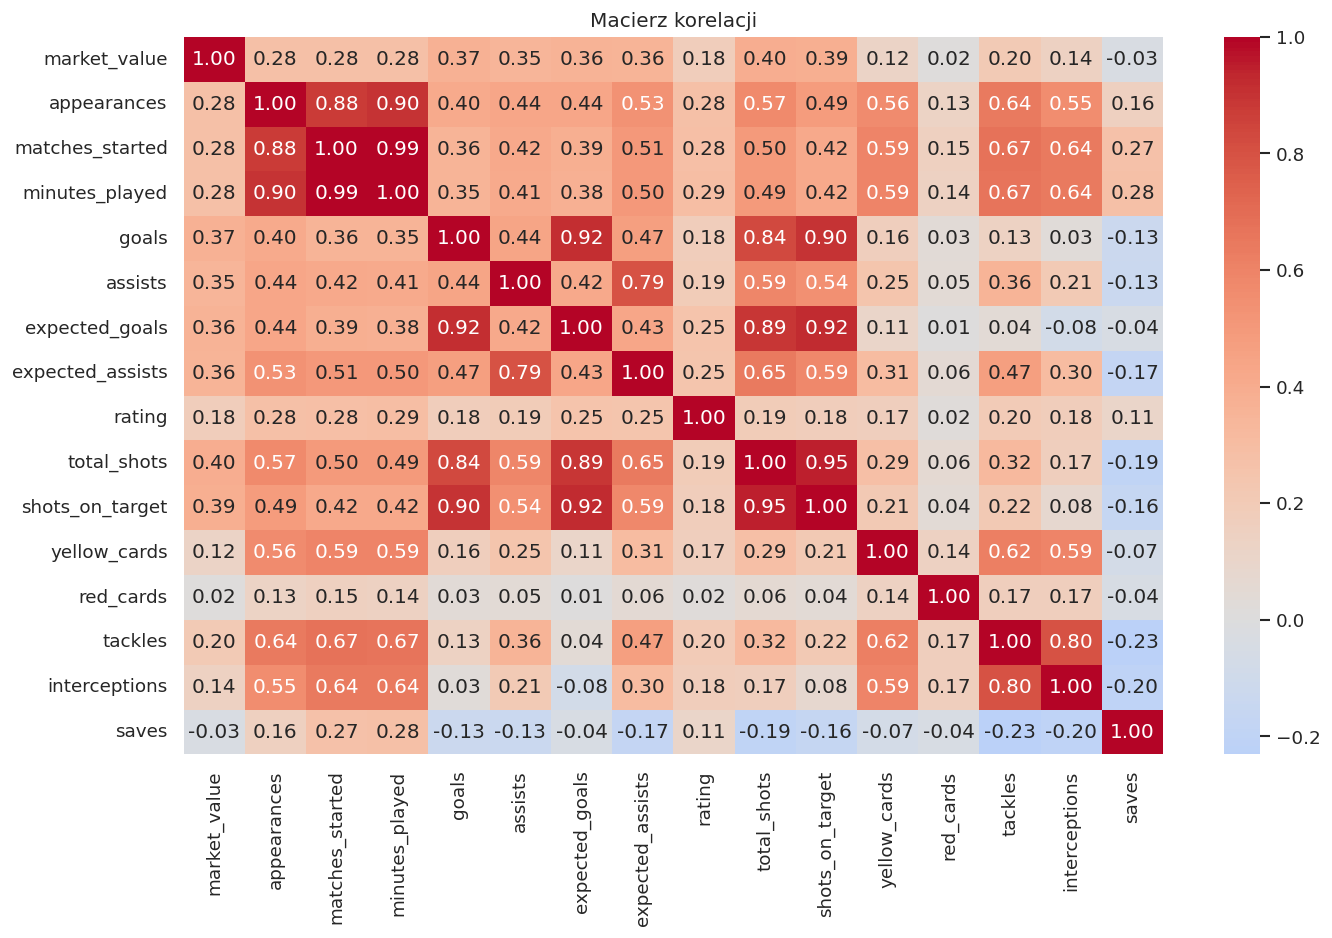
\includegraphics[width=0.9\textwidth]{eda_correlation.png}
    \end{center}
\end{frame}

\begin{frame}{Wnioski z macierzy korelacji}
        \textbf{Silne korelacje dodatnie ($r > 0{,}7$):}
        \begin{itemize}
            \item \texttt{goals} $\leftrightarrow$ \texttt{total\_shots}, \texttt{expected\_goals} - zawodnicy strzelający dużo próbują często i generują dużo xG
            \item \texttt{appearances} $\leftrightarrow$ \texttt{matches\_started} $\leftrightarrow$ \texttt{minutes\_played} - oczywiste, gdyż wszystkie z tych cech mierzą czas gry
            \item \texttt{tackles} $\leftrightarrow$ \texttt{interceptions} - obrońcy aktywni defensywnie
        \end{itemize}

        \vspace{0.5cm}

        \textbf{Korelacje z \texttt{market\_value}:}
        \begin{itemize}
            \item Umiarkowana korelacja z \texttt{goals}, \texttt{rating}, \texttt{appearances}
            \item Brak silnej korelacji z żadną pojedynczą statystyką - wartość rynkowa jest wieloczynnikowa
        \end{itemize}

\end{frame}

\begin{frame}{Statystyki opisowe}
    \small{
    \begin{tabular}{lccccc}
            \toprule
            \textbf{Cecha} & \textbf{Średnia} & \textbf{Std} & \textbf{Min} & \textbf{Mediana} & \textbf{Max} \\
            \midrule
            market\_value (M€) & 9.88 & 16.54 & 0.02 & 3.60 & 218.0 \\
            appearances & 17.72 & 8.99 & 1 & 20 & 32 \\
            minutes\_played & 1149 & 795 & 1 & 1072 & 2880 \\
            goals & 1.56 & 2.68 & 0 & 1 & 31 \\
            assists & 1.10 & 1.69 & 0 & 0 & 18 \\
            expected\_goals & 1.90 & 2.51 & 0.003 & 1.02 & 24.38 \\
            rating & 6.71 & 0.66 & 0 & 6.74 & 9.70 \\
            yellow\_cards & 2.26 & 2.16 & 0 & 2 & 12 \\
            saves & 3.53 & 15.80 & 0 & 0 & 145 \\
            \bottomrule
        \end{tabular}
    }
    \vspace{0.5cm}
    
        Mediana \texttt{market\_value} (3.6M€) jest ponad 2.7× niższa od średniej (9.9M€), \textbf{potwierdza to silne skrzywienie rozkładu}.
    
\end{frame}

%%%
% Preprocessing
%%%

\section{Preprocessing}

\begin{frame}[fragile]{Etapy preprocessingu}
    \begin{columns}
        \column{0.55\textwidth}
        \textbf{Etapy:}
        \begin{enumerate}
            \item \textbf{Filtr aktywności:} $\geq 600$ min $\Rightarrow$ \textbf{2\,580} zawodników
            \item \textbf{Normalizacja do 90 minut}
            \item \textbf{Pipeline num.:} Imputer(median) + StandardScaler
            \item \textbf{Pipeline cat.:} Imputer + OneHotEncoder
            \item Wynik: \textbf{27 cech}, w tym 15 numerycznych.
        \end{enumerate}
        \column{0.45\textwidth}
        \begin{block}{Filtr aktywności}
            Poniżej 600 min (ok. 7 meczów) statystyki są niestabilne, jeden wyjątkowy mecz zaburza profil. Filtr usuwa 1\,169 zawodników (31\%).
        \end{block}
        \begin{block}{Normalizacja}
            Zawodnicy rozgrywający 200 minut i 2000 minut są nieporównywalni w wartościach bezwzględnych. Normalizacja do 90 minut eliminuje wpływ czasu gry.
        \end{block}

    \end{columns}
\end{frame}

%%%
% Klasteryzacja
%%%

\begin{frame}[c]
    \centering
    \vfill
    {\usebeamerfont{frametitle}\usebeamercolor[fg]{frametitle} Klasteryzacja}
    \vfill
\end{frame}

\section{Klasteryzacja}

\begin{frame}{Dobór liczby klastrów}

    \begin{columns}[T]
        \column{0.5\textwidth}
            \begin{center}
                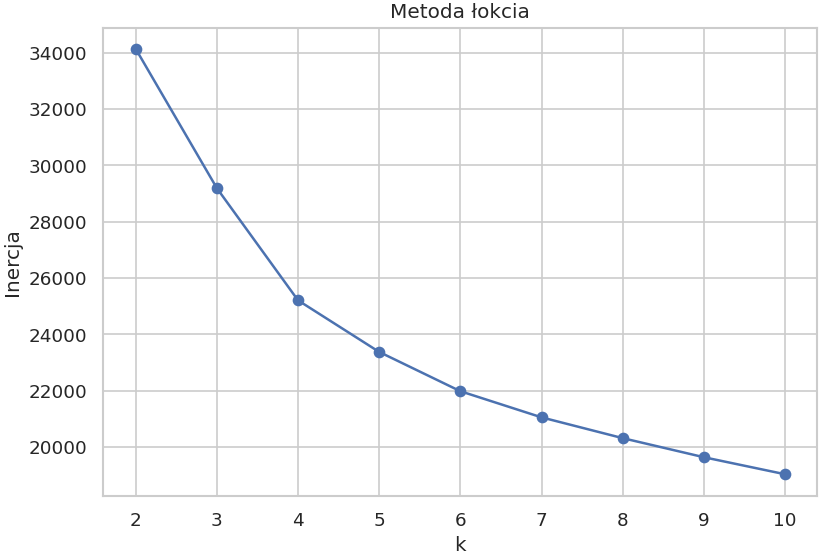
\includegraphics[width=0.95\textwidth]{figures/metoda_lokcia.png}
            
                \textbf{Metoda łokcia:} brak wyraźnego \textit{zagięcia}, spadek równomierny. Typowe dla danych z naturalną hierarchią.
            \end{center}
            
        \column{0.5\textwidth}
            \begin{center}
                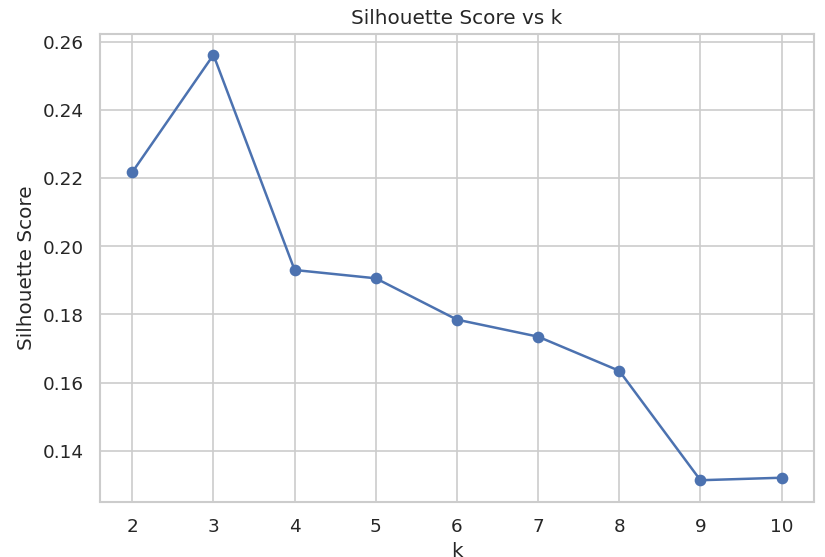
\includegraphics[width=0.95\textwidth]{figures/silhouette.png}
                
                \textbf{Silhouette Score:} maksimum dla $k=3$. Wartość umiarkowana, klastry nachodzą na siebie.
            \end{center}
    \end{columns}
\end{frame}

\begin{frame}{Klastry (KMeans, $k=3$)}

    \small{
    \begin{center}
        \begin{tabular}{lrrrrrr}
            \toprule
            \textbf{Klaster} & \textbf{n} & \textbf{market\_val (M€)} & \textbf{goals} & \textbf{assists} & \textbf{rating} & \textbf{saves} \\
            \midrule
            0 & 1642 & 9.92  & 0.97 & 1.15 & 6.79 & 0.00 \\
            1 & 742  & 19.02 & 5.20 & 2.63 & 6.85 & 0.00 \\
            2 & 196  & 7.51  & 0.01 & 0.10 & 6.98 & 64.48 \\
            \bottomrule
        \end{tabular}
    \end{center}
    }

    \small{
    \begin{center}
        \begin{tabular}{lrrrr}
            \toprule
            \textbf{Klaster} & \textbf{D (\%)} & \textbf{F (\%)} & \textbf{G (\%)} & \textbf{M (\%)} \\
            \midrule
            0 & 54.5 & 2.9  & 0.0   & 42.6 \\
            1 & 0.7  & 56.7 & 0.0   & 42.6 \\
            2 & 0.0  & 0.0  & 100.0 & 0.0  \\
            \bottomrule
        \end{tabular}
    \end{center}
    }

    \vspace{0.3cm}

    \textbf{Klaster 0} - obrońcy i defensywni pomocnicy (niskie gole, niski market value). \textbf{Klaster 1} - napastnicy i ofensywni pomocnicy: 2× wyższa wartość rynkowa. \textbf{Klaster 2} - bramkarze: 100\% G, najwyższy rating, ale najniższa wartość rynkowa.

\end{frame}

\begin{frame}{Wizualizacja PCA}

    \begin{columns}[T]
        \column{0.5\textwidth}
            \begin{center}
                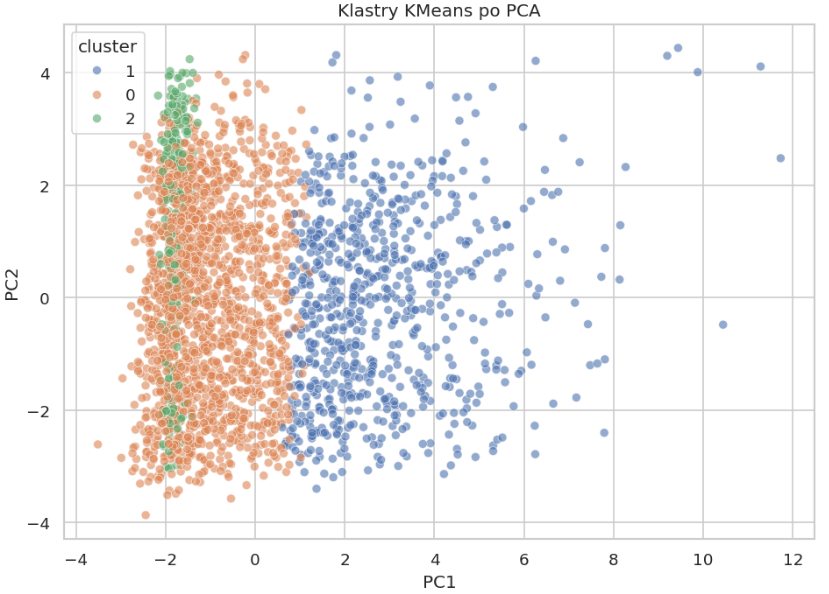
\includegraphics[width=0.95\textwidth]{figures/klastry_pca.png}
                \small \textbf{PC1}: shots, xG, goals\_per90, dobrze rozdziela bramkarzy/obrońców od napastników.
            \end{center}
            
            \column{0.5\textwidth}
            \begin{center}
                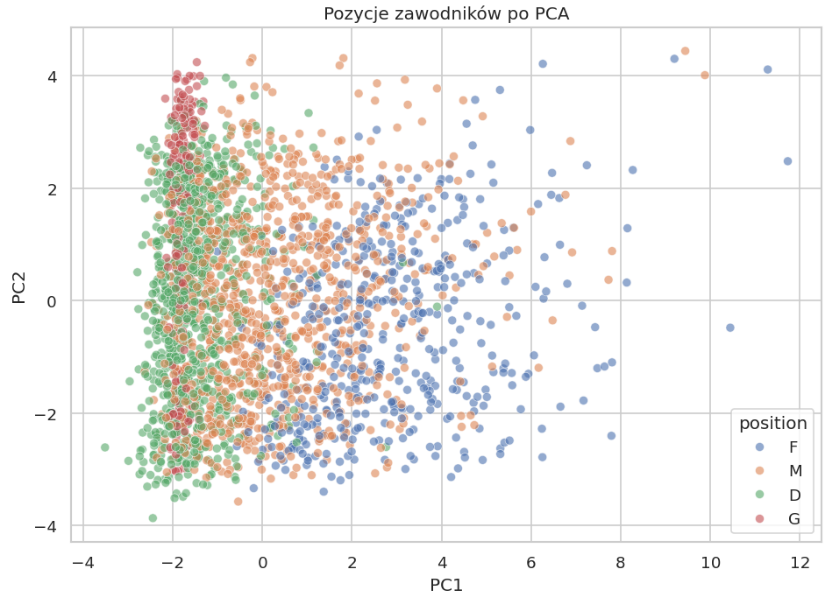
\includegraphics[width=0.95\textwidth]{figures/pozycje_pca.png}
                \small \textbf{PC2}: minuty, starty, mecze, rozdziela rezerwowych od podstawowych graczy.
            \end{center}
    \end{columns}
\end{frame}

\begin{frame}{Wnioski z klasteryzacji}
    \begin{columns}[T]
        \column{0.5\textwidth}
        \textbf{Klaster 0} (obrońcy/pomocnicy):
        \begin{itemize}\small
            \item Nico Schlotterbeck [D] (Bundesliga) 7.69
            \item Manuel Locatelli [M] (Serie A) 7.69
            \item Gonçalo Inácio [D] (Liga Portugal) 7.56
        \end{itemize}
        \textbf{Klaster 2} (bramkarze):
        \begin{itemize}\small
            \item Joël Drommel [G] (Eredivisie) 7.52
            \item Matías Dituro [G] (LaLiga) 7.50
        \end{itemize}
        \column{0.5\textwidth}
        \textbf{Klaster 1} (napastnicy/ofensywni pomocnicy):
        \begin{itemize}\small
            \item Joey Veerman [M] (Eredivisie) 8.00
            \item Lamine Yamal [M] (LaLiga) 7.92
            \item Harry Kane [F] (Bundesliga) 7.92
        \end{itemize}
        \begin{block}{Wniosek}
            KMeans bez wiedzy o pozycjach odtworzył je w ~97\% dla bramkarzy i ~85\% dla napastników. Nierozróżnialność D/M odzwierciedla rzeczywiste zatarcie granic w dzisiejszej grze.
        \end{block}
    \end{columns}
\end{frame}

%%%
% Regresja
%%%

\section{Regresja}

\begin{frame}[c]
    \centering
    \vfill
    {\usebeamerfont{frametitle}\usebeamercolor[fg]{frametitle} Regresja}
    \vfill
\end{frame}

\begin{frame}[fragile]{Cel i pipeline regresji}
    \begin{columns}[T]
        \column{0.55\textwidth}
            \begin{block}{Cel}
                \textbf{Cel:} przewidywanie wartości rynkowej (\texttt{market\_value}) na podstawie statystyk meczowych.
            \end{block}
    
            \vspace{0.5cm}
            
            \textbf{Transformacja celu:} $y = \ln(1 + \text{market\_value})$ \\ \\
            Logarytmizacja redukuje wpływ outlierów i sprawia, że błędy modelu są proporcjonalne, a nie bezwzględne, np. błąd 1M€ przy graczu o wartości 2M€ to inny problem niż przy graczu o wartości 150M€.

        \column{0.42\textwidth}
            \begin{block}{Pipeline}
                \begin{enumerate}
                    \item SimpleImputer (median)
                    \item StandardScaler
                    \item OneHotEncoder (\texttt{position})
                    \item LinearRegression
                \end{enumerate}
            \end{block}
            
            \vspace{0.5cm}
            
            Podział: \textbf{80/20}, random\_state=42.\\
            Próbki po usunięciu NaN w target: ok.~2\,450.

    \end{columns}
\end{frame}

\begin{frame}{Metryki modeli}
    \begin{center}
        \begin{tabular}{lrrrr}
            \toprule
            \textbf{Model} & \textbf{R² train} & \textbf{R² test} & \textbf{MAE test (log)} \\
            \midrule
            \textbf{LinearRegression} & \textbf{0.220} & \textbf{0.143} & \textbf{1.032} \\
            Ridge($\alpha$=1.0)       & 0.220 & 0.142 & 1.033 \\
            Lasso($\alpha$=0.01)      & 0.211 & 0.137 & 1.042 \\
            Ridge($\alpha$=10.0)      & 0.219 & 0.137 & 1.037 \\
            Lasso($\alpha$=0.1)       & 0.186 & 0.136 & 1.054 \\
            \bottomrule
        \end{tabular}
    \end{center}
    
    \vspace{0.3cm}
    
    \begin{columns}
        \column{0.5\textwidth}
        \begin{block}{Regularyzacja nie pomaga}
            Wyniki train $\approx$ test, model \textbf{nie jest przeuczony}. Regularyzacja nie poprawia wyników, bo problemem jest \textbf{underfitting}, nie overfitting.
        \end{block}
        \column{0.5\textwidth}
        \begin{alertblock}{Dlaczego R² = 0.14?}
            Wartość rynkowa zależy od: wieku, długości kontraktu, marketingu, popularności, potencjału, cech tych brakuje w datasecie.
        \end{alertblock}
    \end{columns}
\end{frame}

\begin{frame}{Porównanie modeli (Actual vs Predicted)}
    \begin{center}
        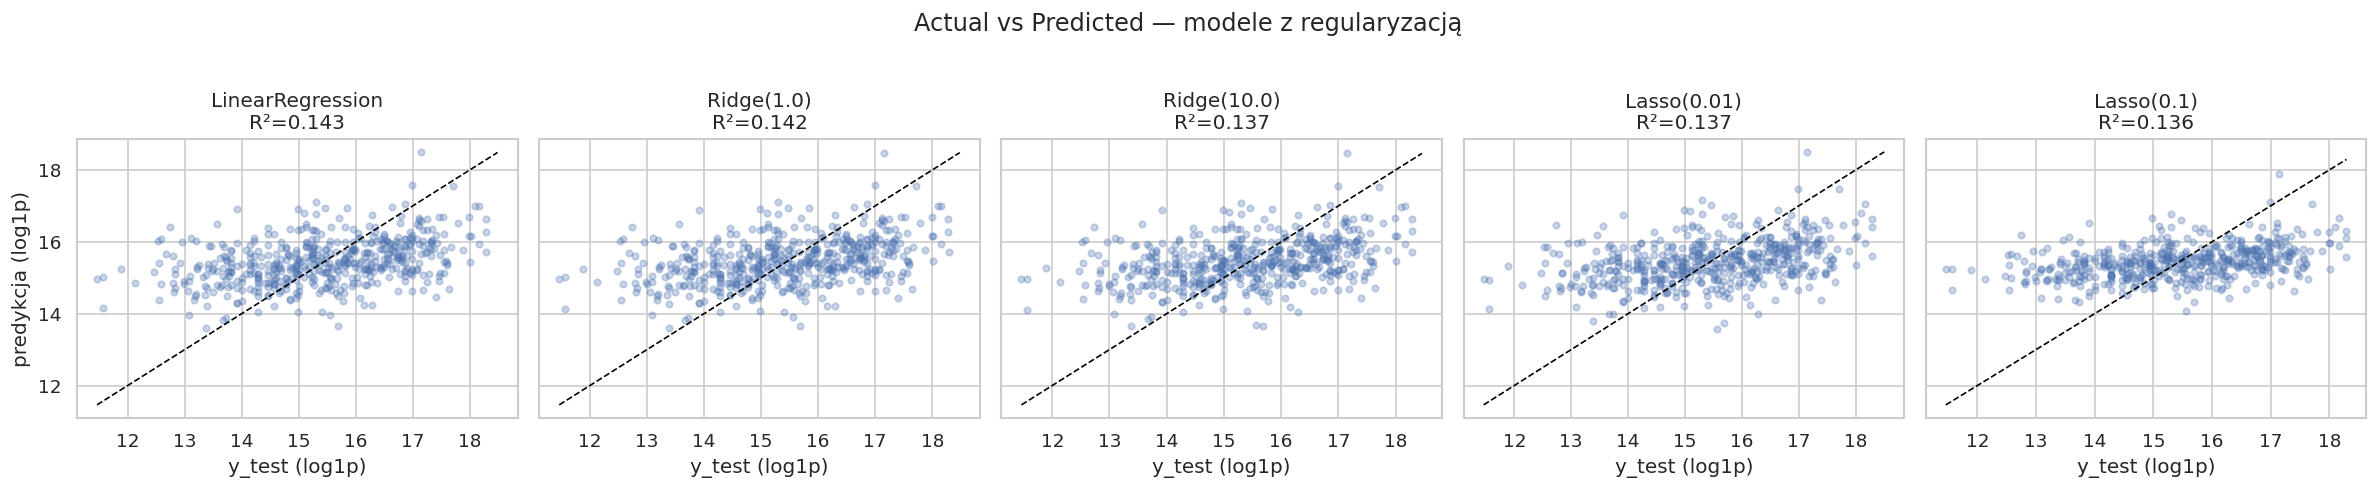
\includegraphics[width=1\textwidth]{regression_comparison.png}
    \end{center}

    \vspace{0.3cm}
    
    Wszystkie modele mają zbliżony kształt chmury punktów. Potwierdzony brak systematycznej poprawy od regularyzacji. Duże rozrzuty w obszarze wysokich wartości (gwiazdy) są trudne do uchwycenia bez dodatkowych cech.
\end{frame}

\begin{frame}{Współczynniki regresji liniowej}
    \begin{columns}[T]
        \column{0.4\textwidth}
            \small{
            \begin{itemize}
                \item \textbf{Dodatnie:} \texttt{position\_G} (+1.63), \texttt{rating} (+0.51), \texttt{expected\_goals\_per90} (+0.31), \texttt{appearances} (+0.24) - regularność gry i kreowanie sytuacji podnoszą wycenę.
                \item \textbf{Ujemne:} \texttt{saves\_per90} (-0.70), \texttt{position\_F} (-0.36), \texttt{position\_M} (-0.21).
                \item \textbf{Współliniowość:} \texttt{position\_G} i \texttt{saves\_per90} działają łącznie - tylko bramkarze mają \texttt{saves}$\neq$0, więc efekt netto dla bramkarza jest \textbf{ujemny}. Stąd bramkarze wyceniani najniżej (klaster 2: 7.51M€).
            \end{itemize}
            }

        \column{0.7\textwidth}
            \begin{center}
                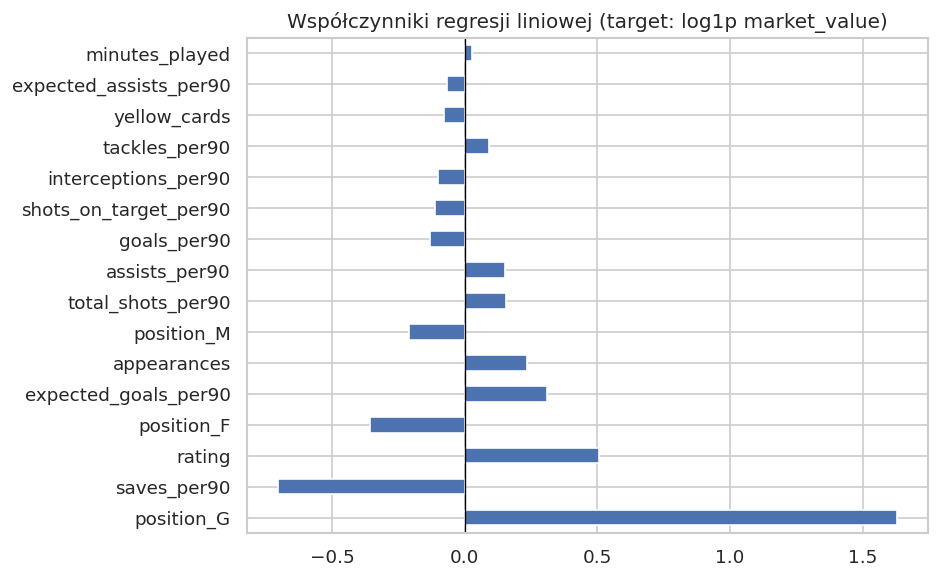
\includegraphics[width=\textwidth]{regression_coefs.png}
            \end{center}
    \end{columns}

\end{frame}

\begin{frame}{Reszty modelu — kogo wycena rynkowa zaskakuje?}
    \begin{center}
        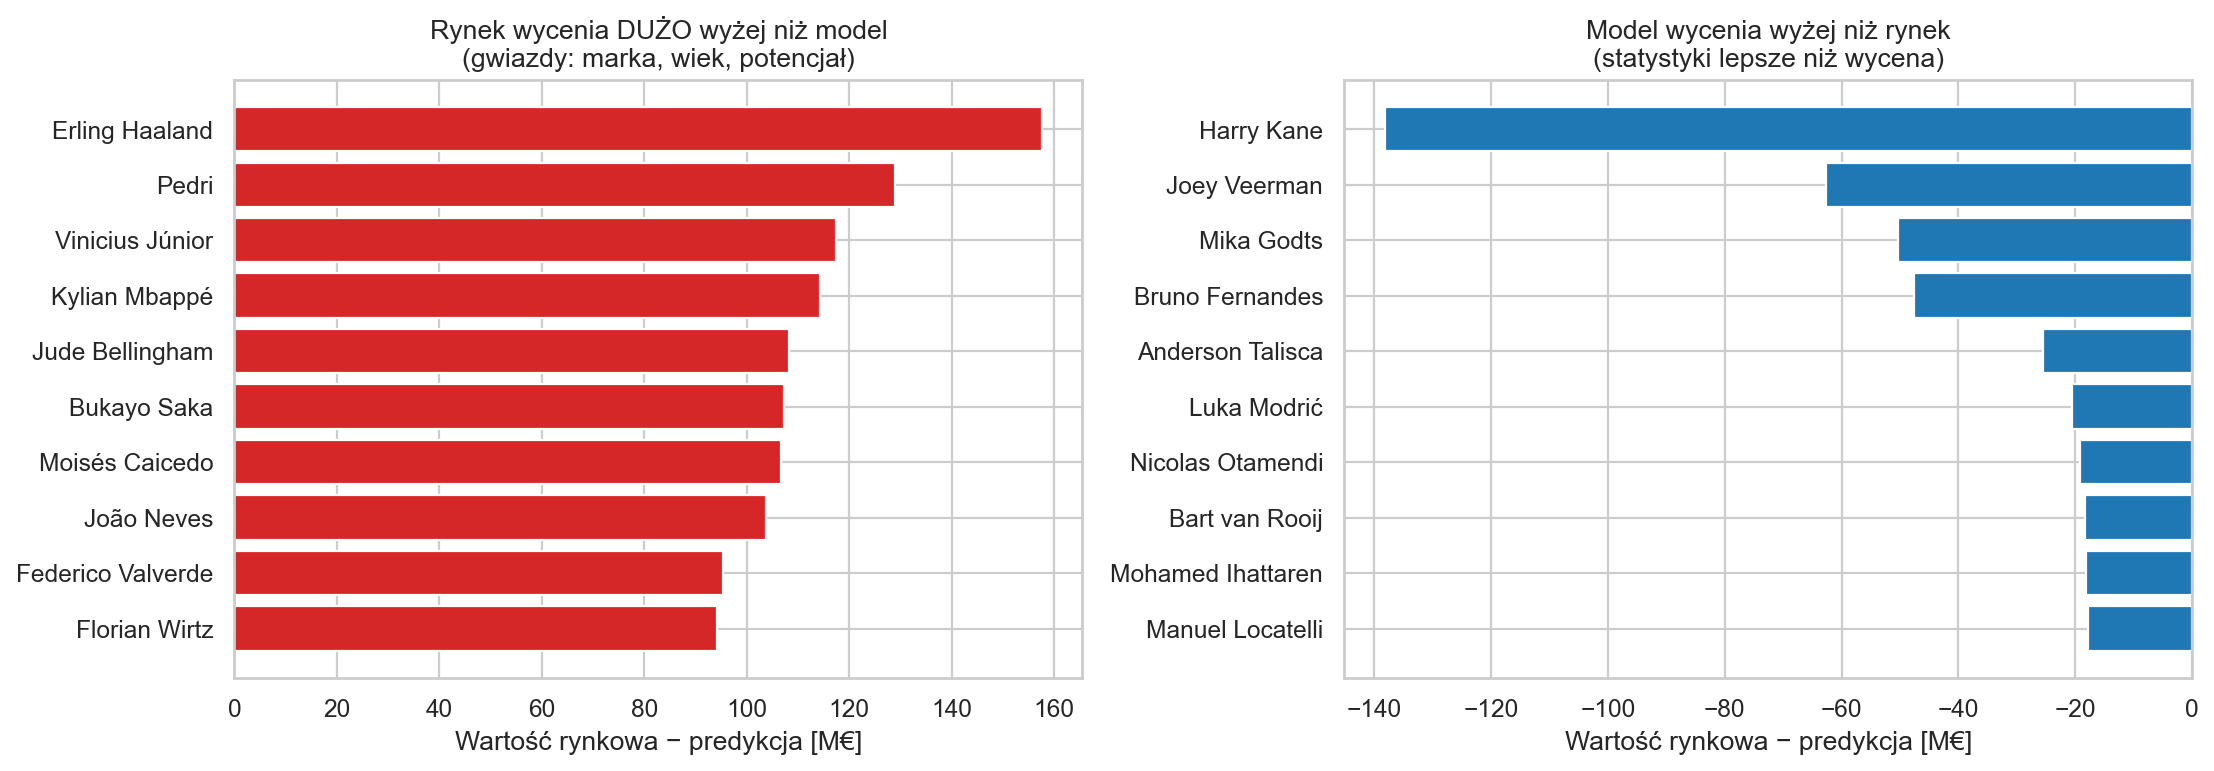
\includegraphics[width=0.82\textwidth]{regression_residuals.png}
    \end{center}
    \vspace{0.1cm}
    \begin{columns}[T]
        \column{0.5\textwidth}
        \small{\textbf{Rynek $>$ model} (niedoszacowani): \textbf{młode gwiazdy} (Haaland, Pedri, Vinícius, Mbappé, Bellingham) — rynek płaci za \textbf{potencjał i markę}, których statystyki nie widzą.}
        \column{0.5\textwidth}
        \small{\textbf{Model $>$ rynek} (przeszacowani): \textbf{starsi zawodnicy} (Kane, Modrić, B. Fernandes) — świetne statystyki, ale rynek dyskontuje \textbf{wiek}.}
    \end{columns}
    \vspace{0.15cm}
    \textbf{Wniosek:} największe błędy układają się wzdłuż brakującej cechy — \textbf{wieku}. To tłumaczy niskie $R^2$ lepiej niż sama metryka.
\end{frame}

%%%
% Klasyfikacja
%%%

\begin{frame}[c]
    \centering
    \vfill
    {\usebeamerfont{frametitle}\usebeamercolor[fg]{frametitle} Klasyfikacja}
    \vfill
\end{frame}

\section{Klasyfikacja}

\begin{frame}{Cel i metodologia}
    \begin{block}{Cel}
        przewidywanie pozycji zawodnika (F/M/D/G) wyłącznie na podstawie statystyk meczowych, bez informacji o pozycji w danych wejściowych.
    \end{block}

    \vspace{0.3cm}
    \textbf{Strategia:} OneVsRestClassifier dla każdego modelu. Preprocessing: SimpleImputer(median) + MinMaxScaler.

    \vspace{0.3cm}
    \begin{tabular}{lrrrr}
        \toprule
        \textbf{Model} & \textbf{Acc train} & \textbf{Acc test} & \textbf{Precision} & \textbf{Recall} \\
        \midrule
        LogisticRegression     & 0.698 & 0.679 & 0.764 & 0.681 \\
        \textbf{SVC}           & \textbf{0.728} & \textbf{0.724} & \textbf{0.772} & \textbf{0.775} \\
        KNeighborsClassifier   & 0.777 & 0.652 & 0.720 & 0.703 \\
        DecisionTreeClassifier & 1.000 & 0.563 & 0.665 & 0.661 \\
        RandomForestClassifier & 1.000 & 0.705 & 0.774 & 0.751 \\
        \bottomrule
    \end{tabular}
\end{frame}

\begin{frame}{Porównanie modeli}
    
    \begin{columns}[T]
        \column{0.4\textwidth}
        \begin{alertblock}{SVC (72.4\%)}
            SVM dobrze radzi sobie z nieliniowymi granicami decyzyjnymi między pozycjami. Stabilny: train 72.8\% vs test 72.4\%, brak przeuczenia, \textbf{najlepszy model}.
        \end{alertblock}
        
        \begin{alertblock}{RandomForest (70.5\%)}
            Dobry wynik mimo 100\% na treningu, ensemble zmniejsza wariancję. Precision 77.4\% to najwyższy wynik spośród modeli.
        \end{alertblock}
        
        \column{0.58\textwidth}

        \begin{alertblock}{LogisticRegression (67.9\%)}
            Porównywalne wyniki na zbiorze train (69.8\%) i zbiorze testowym (67.9\%), ale słabsze od SVC i RandomForest.
        \end{alertblock}
        
        \begin{alertblock}{DecisionTree (56.3\%)}
            100\% na treningu, 56.3\% na teście. Drzewo bez ograniczenia głębokości zapamiętuje szum zamiast wzorców, \textbf{duży problem z przeuczeniem}.
        \end{alertblock}
        
        \begin{alertblock}{KNN (65.2\%)}
            Wysoki train acc (77.7\%) nie przekłada się na test (65.2\%), \textbf{przeuczenie}.
        \end{alertblock}
    \end{columns}
\end{frame}

\begin{frame}{Macierz błędów (SVC, zbiór testowy)}
    \begin{columns}[T]
        \column{0.45\textwidth}
            \begin{center}
                \begin{itemize}
                    \item \textbf{G (bramkarze):} klasyfikowani niemal bezbłędnie, cecha \texttt{saves} jest unikalnym sygnałem
                    \item \textbf{F (napastnicy):} wysoka precyzja; rzadkie pomyłki z M.
                    \item \textbf{M $\leftrightarrow$ D:} najczęstsze błędy, obrońcy grający wysoko i pomocnicy defensywni mają podobne statystyki.
                \end{itemize}
            \end{center}

        \column{0.6\textwidth}
            \begin{center}
                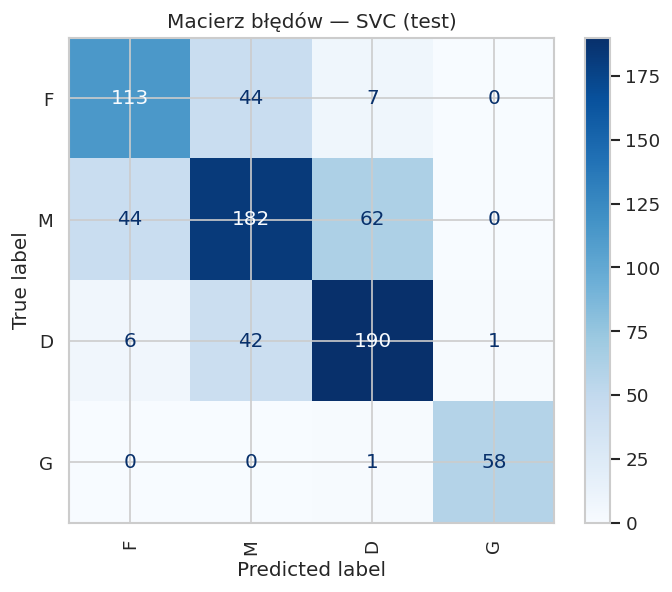
\includegraphics[width=0.95\textwidth]{classification_cm.png}
            \end{center}
    \end{columns}

\end{frame}

\begin{frame}{Ważność cech — które statystyki definiują pozycję?}
    \begin{columns}[T]
        \column{0.55\textwidth}
            \begin{center}
                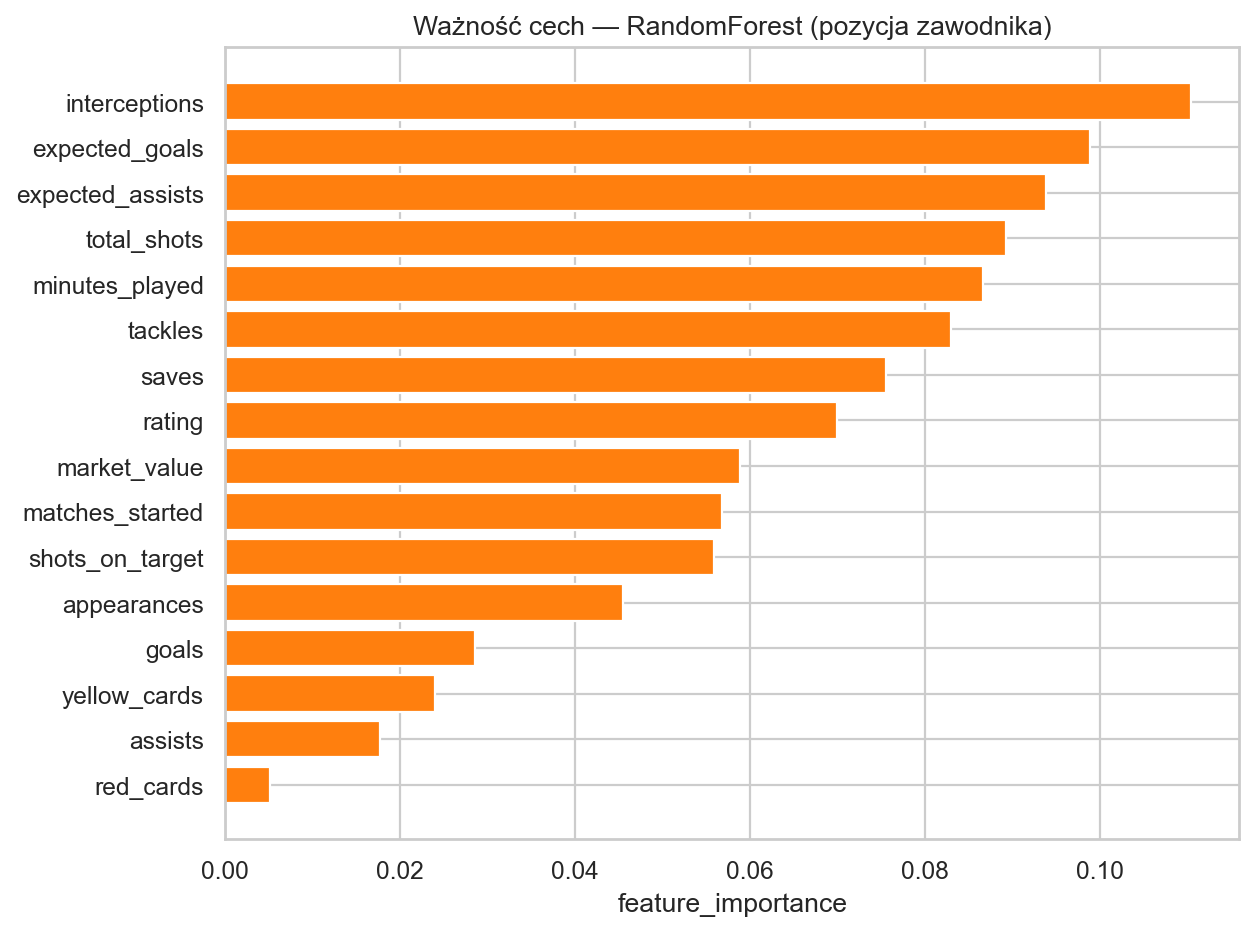
\includegraphics[width=0.95\textwidth]{classification_importances.png}
            \end{center}
        \column{0.45\textwidth}
            \small{
            \begin{itemize}
                \item Ważność rozkłada się \textbf{równomiernie} — pozycja to cecha \textbf{wielowymiarowa}, nie wynika z jednej statystyki.
                \item \texttt{interceptions}, \texttt{tackles} → sygnał \textbf{defensywny} (D)
                \item \texttt{expected\_goals}, \texttt{total\_shots} → sygnał \textbf{ofensywny} (F)
                \item \texttt{saves} → unikalny marker \textbf{bramkarzy} (G)
            \end{itemize}
            }
            \vspace{0.2cm}
            \small{Spójne z macierzą błędów: G rozpoznawani niemal bezbłędnie, D$\leftrightarrow$M mylone (te same cechy defensywne).}
    \end{columns}
\end{frame}

%%%
% Hipotezy
%%%

\begin{frame}[c]
    \centering
    \vfill
    {\usebeamerfont{frametitle}\usebeamercolor[fg]{frametitle} Hipotezy}
    \vfill
\end{frame}

\section{Weryfikacja hipotez statystycznych}

\begin{frame}{Hipoteza 1: Napastnicy vs Pomocnicy}

    \begin{columns}[T]
        \column{0.48\textwidth}
        
            \textbf{Pytanie:} Czy napastnicy strzelają istotnie więcej bramek na 90 minut niż pomocnicy?

            \vspace{0.2cm}
            
            \textbf{Hipotezy:}
            \begin{itemize}
                \item $H_0$: rozkłady \texttt{goals/90} są identyczne (mediany równe)
                \item $H_1$: napastnicy mają wyższe \texttt{goals/90} (test jednostronny)
            \end{itemize}
        
            \vspace{0.2cm}
        
            \small{
                \begin{tabular}{lrrr}
                    \toprule
                    Grupa & n & Mediana & Średnia \\
                    \midrule
                    Forwards (F)    & 469  & 0.294 & 0.333 \\
                    Midfielders (M) & 1015 & 0.093 & 0.126 \\
                    \bottomrule
                \end{tabular}
            }

        \column{0.52\textwidth}
            \begin{center}
                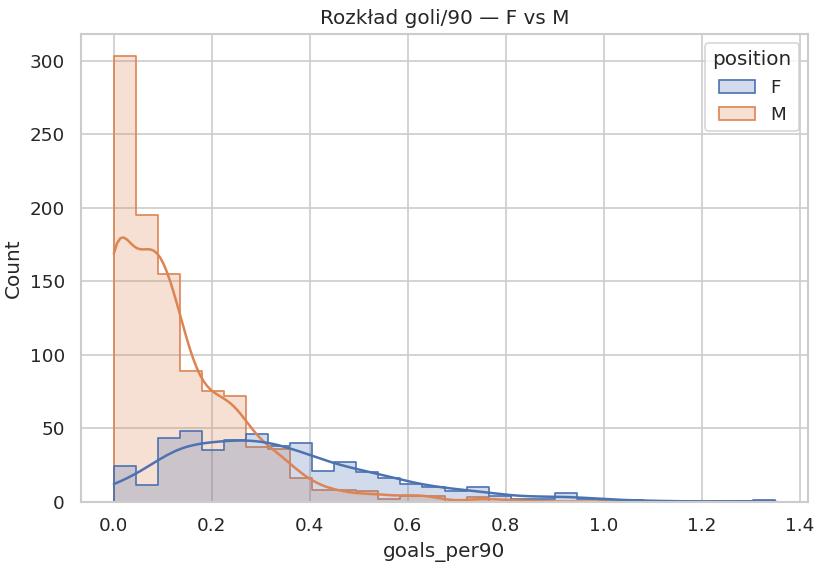
\includegraphics[width=0.8\textwidth]{figures/rozklad_goli_90.png}
                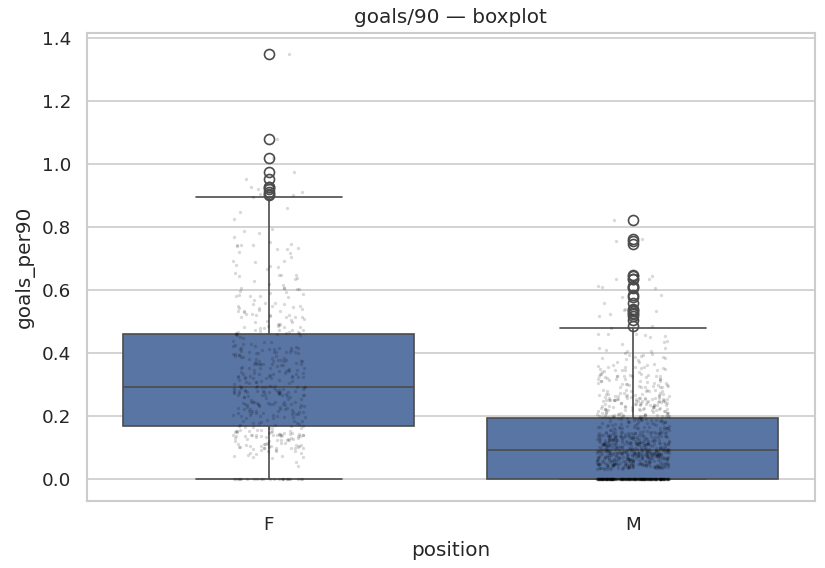
\includegraphics[width=0.8\textwidth]{figures/golas90.png}
            \end{center}
    \end{columns}
\end{frame}

\begin{frame}{Wyniki testów statystycznych}
    \textbf{Shapiro-Wilk:} oba rozkłady \textbf{nienormalne} i prawostronne, z długim ogonem. Uzasadnia użycie testu nieparametrycznego.

    \vspace{0.2cm}
    \textbf{Test U Manna-Whitneya} (jednostronny F $>$ M):
    \begin{itemize}
        \item $p \approx 0{,}000000 \ll 0.05$
        \item \textbf{Odrzucamy $H_0$}
    \end{itemize}

    \vspace{0.2cm}
    \textbf{Bootstrap 95\% CI} dla różnicy median (F $-$ M):
    \begin{itemize}
        \item CI $=$ [0.1829,\ 0.2318]
        \item Obserwowana różnica $=$ 0.2008
        \item CI \textbf{nie zawiera zera}
    \end{itemize}
    \begin{block}{Wniosek}
        Statystycznie istotna różnica. Napastnik strzelający \textbf{0.20 gola/90 min} więcej niż pomocnik.
    \end{block}
\end{frame}

\begin{frame}{Bootstrap - wykres rozkładu}
    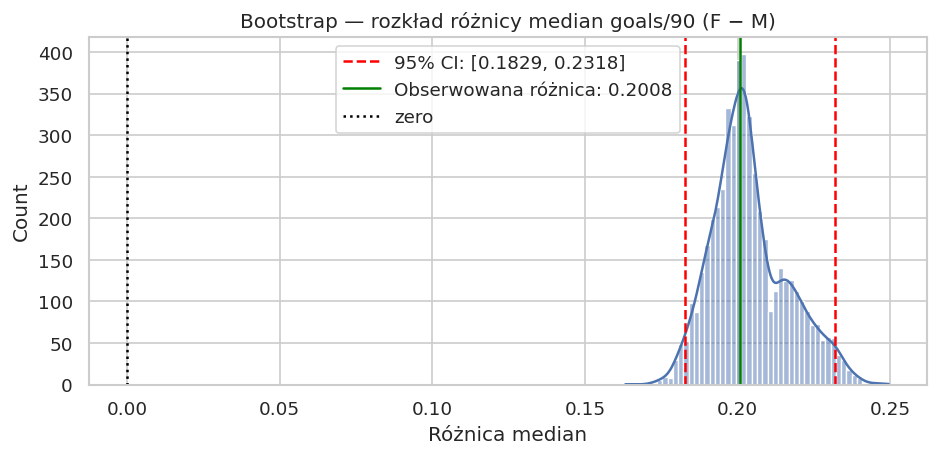
\includegraphics[width=\textwidth]{hyp1_bootstrap.png}
\end{frame}

\begin{frame}{Hipoteza 2: Premier League vs pozostałe ligi (rating)}
    \begin{columns}
        \column{0.52\textwidth}
            \textbf{Pytanie:} Czy zawodnicy Premier League mają istotnie inny rating niż zawodnicy z pozostałych lig?

            \vspace{0.2cm}
            
            \textbf{Hipotezy:}
            \begin{itemize}
                \item $H_0$: średni rating PL = średni rating innych lig
                \item $H_1$: rating różny (test dwustronny)
            \end{itemize}
            
            \vspace{0.2cm}
        
            \begin{tabular}{lrrr}
                \toprule
                Grupa & n & Średnia & Mediana \\
                \midrule
                Premier League  & 355  & 6.823 & 6.809 \\
                Pozostałe ligi  & 2225 & 6.825 & 6.800 \\
                \bottomrule
            \end{tabular}
        \column{0.48\textwidth}
            \begin{center}
                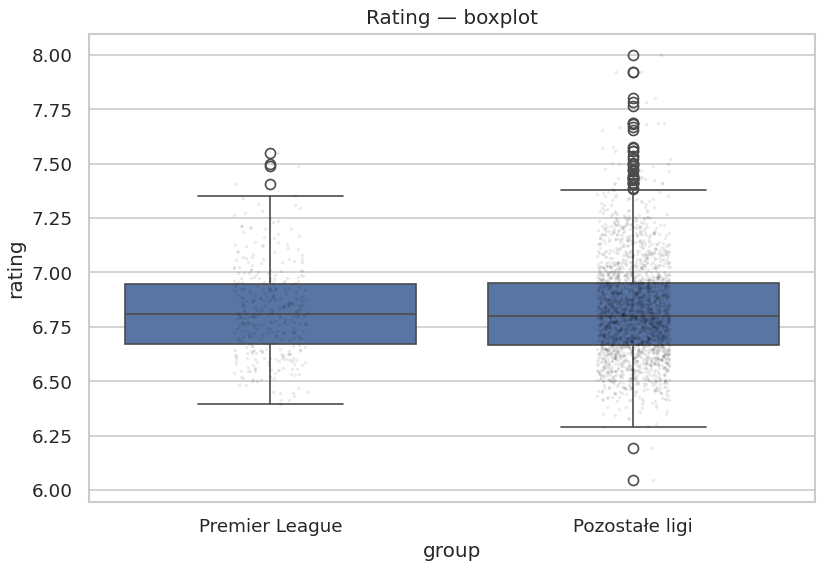
\includegraphics[width=0.85\textwidth]{figures/rating_boxplot.png}
                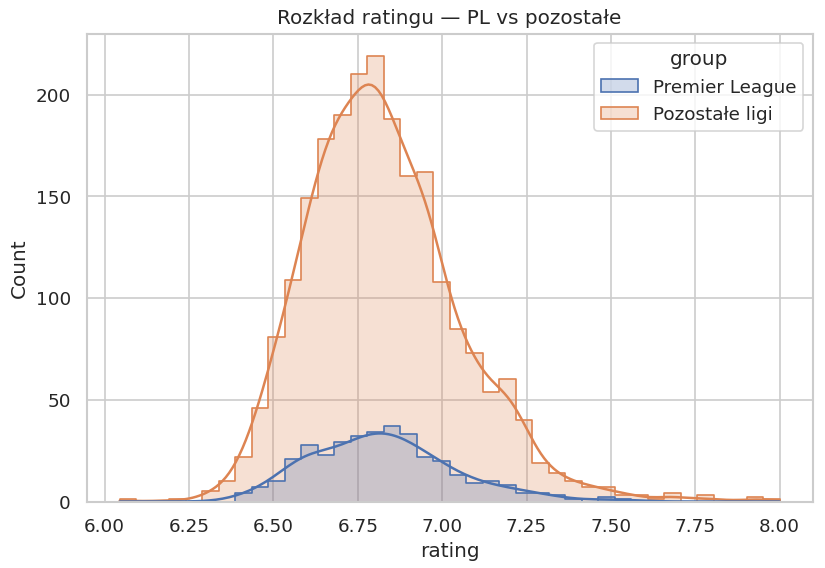
\includegraphics[width=0.85\textwidth]{figures/rozklad_ratingu_pl.png}
            \end{center}
    \end{columns}
\end{frame}

\begin{frame}{Wyniki testów statystycznych}
    \begin{columns}[T]
        \column{0.55\textwidth}
        \textbf{Shapiro-Wilk:} rozkłady \textbf{nienormalne} ($p \ll 0.05$).\\

        \vspace{0.2cm}
        
        \textbf{Levene:} nierówne wariancje → Welch t-test zamiast klasycznego t-testu.

        \vspace{0.3cm}
        
        \begin{tabular}{lrr}
            \toprule
            \textbf{Test} & \textbf{p-value} & \textbf{Istotny?} \\
            \midrule
            Welch t-test   & 0.9084 & Nie \\
            Mann-Whitney U & 0.8684 & Nie \\
            \bottomrule
        \end{tabular}

        \vspace{0.3cm}
        
        \textbf{95\% CI dla różnicy średnich:} zawiera zero.
        
        \column{0.45\textwidth}
        \begin{alertblock}{Wniosek}
            \textbf{Brak podstaw do odrzucenia $H_0$.} Rating piłkarzy Premier League nie różni się istotnie od ratingu z innych lig.
        \end{alertblock}
        \begin{block}{Interpretacja}
            Rating jest normalizowany wewnątrz meczu, wyższy poziom ligi nie przekłada się na wyższe oceny.
        \end{block}
    \end{columns}
\end{frame}

\begin{frame}{Porównanie lig — wartość rynkowa vs rating}
    \begin{center}
        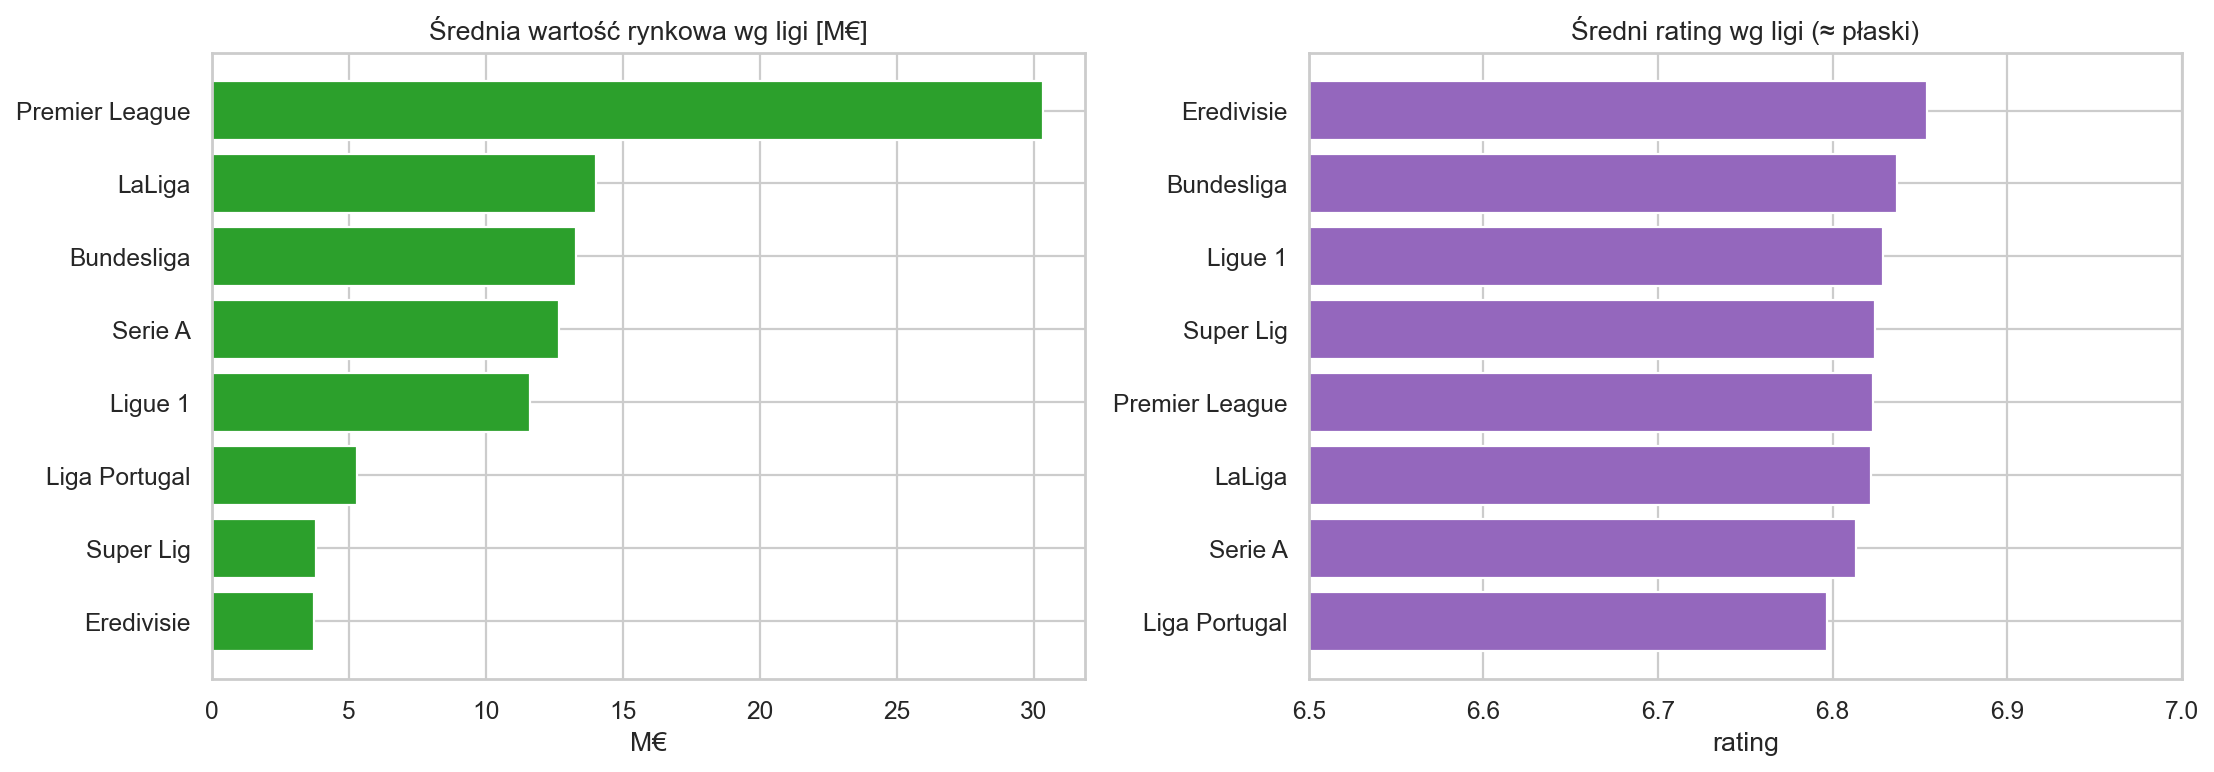
\includegraphics[width=0.95\textwidth]{league_comparison.png}
    \end{center}
    \vspace{0.1cm}
    \begin{columns}[T]
        \column{0.5\textwidth}
        \small{\textbf{Wartość rynkowa} skrajnie zróżnicowana: Premier League ($\approx$30M€) to ok.~8× Eredivisie/Super Lig ($\approx$3.7M€).}
        \column{0.5\textwidth}
        \small{\textbf{Rating} praktycznie płaski (6.80–6.85) we wszystkich ligach.}
    \end{columns}
    \vspace{0.15cm}
    \begin{block}{Spójne z Hipotezą 2}
        Rating jest normalizowany wewnątrz ligi/meczu, więc nie odróżnia poziomu rozgrywek — potwierdza to brak istotnej różnicy PL vs reszta.
    \end{block}
\end{frame}


\begin{frame}{Ogólne wnioski o badanym zbiorze}
    \begin{center}
        \begin{itemize}
            \item Statystyki meczowe \textbf{dobrze opisują rolę zawodnika} (pozycja, klaster), ale \textbf{słabo tłumaczą jego wartość rynkową}, brakuje cech pozaboiskowych takich jak przykładowo kontrakt, marka osobista.
            \item Systemy oceniania (rating) są \textbf{relatywne ligowo}, a więc porównania między ligami wymagają dodatkowej standaryzacji.
            \item Przy wielowymiarowych danych sportowych nawet proste modele (regresja logistyczna, KMeans) dają interpretowalne i sensowne wyniki.
        \end{itemize}
    \end{center}
\end{frame}

\begin{frame}{Dziękujemy za uwagę}
    Linki i odnośniki:
    \begin{itemize}
        \item \href{https://www.kaggle.com/datasets/kaanyorgun/european-top-leagues-player-stats-25-26}{Zbiór danych, Kaggle}
        \item \href{https://github.com/wojciechbukala/FootballPlayersAnalysis}{Repozytorium projektowe, GitHub}
    \end{itemize}
    
\end{frame}

\end{document}
